\documentclass[12pt]{article}
\usepackage[letterpaper, top=17mm, bottom=16mm, left=13mm, right=13mm, headheight=15pt, headsep=4mm, footskip=8mm]{geometry}
\usepackage[T1]{fontenc}
\usepackage{helvet}
\renewcommand{\familydefault}{\sfdefault}
\usepackage{tikz}
\usetikzlibrary{arrows.meta, decorations.markings}
\tikzset{midarrow/.style={postaction={decorate}, decoration={markings, mark=at position 0.5 with {\arrow{Stealth[length=3.6mm, width=3.2mm]}}}}}
\tikzset{smallarrow/.style={postaction={decorate}, decoration={markings, mark=at position 0.5 with {\arrow{Stealth[length=2.6mm, width=2.3mm]}}}}}
\tikzset{bigarrow/.style={-{Stealth[length=3mm, width=2.6mm]}, line width=1.1pt}}
\usepackage{fancyhdr}
\pagestyle{fancy}
\fancyhf{}
\lhead{\normalsize Week 62 / Conflict networks / K--1}
\lfoot{\small Bellingham Math Circle / Week 62 / W62-RV-K-v1}
\rfoot{\small \thepage}
\renewcommand{\headrulewidth}{0pt}
\setlength{\parindent}{0pt}
\setlength{\parskip}{0pt}
\raggedright
\begin{document}
\noindent\begin{minipage}[c]{0.64\linewidth}\raggedright The headers show which colour goes with each number. Put one counter on each circle. Two circles joined by a line must not have the same number. The numbers next to a circle show which counters it may have.\end{minipage}\hfill\begin{minipage}[c]{0.33\linewidth}\raggedleft 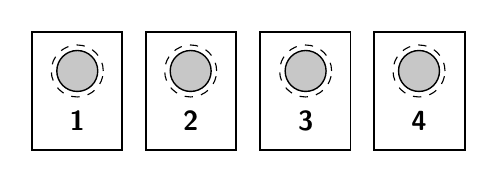
\begin{tikzpicture}[x=1mm, y=1mm]
\useasboundingbox (-0.5,-0.5) rectangle (55.5,15.5);
\draw[line width=0.7pt, fill=white] (0.0,0.0) rectangle (11.5,15.0);
\draw[dashed, line width=0.4pt] (5.8,10.0) circle (3.3mm);
\draw[line width=0.5pt, fill=black!22] (5.8,10.0) circle (2.6mm);
\node[font=\bfseries] at (5.8,3.6) {1};
\draw[line width=0.7pt, fill=white] (14.5,0.0) rectangle (26.0,15.0);
\draw[dashed, line width=0.4pt] (20.2,10.0) circle (3.3mm);
\draw[line width=0.5pt, fill=black!22] (20.2,10.0) circle (2.6mm);
\node[font=\bfseries] at (20.2,3.6) {2};
\draw[line width=0.7pt, fill=white] (29.0,0.0) rectangle (40.5,15.0);
\draw[dashed, line width=0.4pt] (34.8,10.0) circle (3.3mm);
\draw[line width=0.5pt, fill=black!22] (34.8,10.0) circle (2.6mm);
\node[font=\bfseries] at (34.8,3.6) {3};
\draw[line width=0.7pt, fill=white] (43.5,0.0) rectangle (55.0,15.0);
\draw[dashed, line width=0.4pt] (49.2,10.0) circle (3.3mm);
\draw[line width=0.5pt, fill=black!22] (49.2,10.0) circle (2.6mm);
\node[font=\bfseries] at (49.2,3.6) {4};
\end{tikzpicture}\end{minipage}\par
\vspace{5mm}
\noindent\makebox[\linewidth][c]{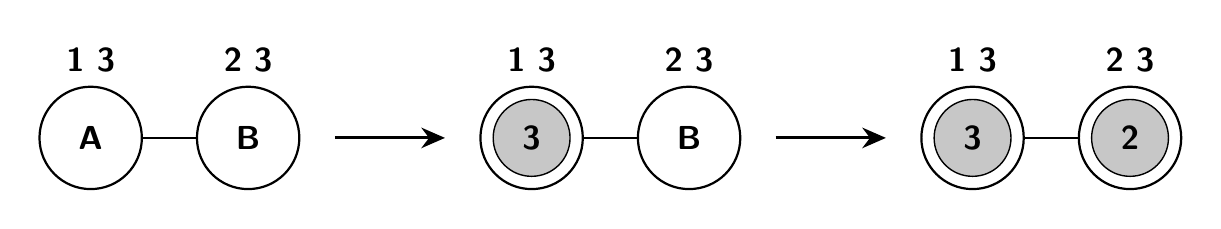
\begin{tikzpicture}[x=1mm, y=1mm]
\useasboundingbox (-8.0,-8.0) rectangle (140.0,14.0);
\draw[line width=0.8pt] (0.00,0.00) -- (20.00,0.00);
\draw[line width=0.8pt, fill=white] (0.00,0.00) circle (6.5mm);
\node[font=\large\bfseries] at (0.00,0.00) {A};
\draw[line width=0.8pt, fill=white] (20.00,0.00) circle (6.5mm);
\node[font=\large\bfseries] at (20.00,0.00) {B};
\node[font=\large\bfseries, inner sep=0.5mm, anchor=270] at (0.00,7.90) {1\,\,3};
\node[font=\large\bfseries, inner sep=0.5mm, anchor=270] at (20.00,7.90) {2\,\,3};
\draw[bigarrow] (31.0,0) -- (45.0,0);
\draw[line width=0.8pt] (56.00,0.00) -- (76.00,0.00);
\draw[line width=0.8pt, fill=white] (56.00,0.00) circle (6.5mm);
\draw[line width=0.5pt, fill=black!22] (56.00,0.00) circle (4.88mm);
\node[font=\large\bfseries] at (56.00,0.00) {3};
\draw[line width=0.8pt, fill=white] (76.00,0.00) circle (6.5mm);
\node[font=\large\bfseries] at (76.00,0.00) {B};
\node[font=\large\bfseries, inner sep=0.5mm, anchor=270] at (56.00,7.90) {1\,\,3};
\node[font=\large\bfseries, inner sep=0.5mm, anchor=270] at (76.00,7.90) {2\,\,3};
\draw[bigarrow] (87.0,0) -- (101.0,0);
\draw[line width=0.8pt] (112.00,0.00) -- (132.00,0.00);
\draw[line width=0.8pt, fill=white] (112.00,0.00) circle (6.5mm);
\draw[line width=0.5pt, fill=black!22] (112.00,0.00) circle (4.88mm);
\node[font=\large\bfseries] at (112.00,0.00) {3};
\draw[line width=0.8pt, fill=white] (132.00,0.00) circle (6.5mm);
\draw[line width=0.5pt, fill=black!22] (132.00,0.00) circle (4.88mm);
\node[font=\large\bfseries] at (132.00,0.00) {2};
\node[font=\large\bfseries, inner sep=0.5mm, anchor=270] at (112.00,7.90) {1\,\,3};
\node[font=\large\bfseries, inner sep=0.5mm, anchor=270] at (132.00,7.90) {2\,\,3};
\end{tikzpicture}}\par
\vspace{5mm}
\textbf{Problem 1:} Put a counter on every circle.\par
\vspace{4mm}
\noindent\makebox[\linewidth][s]{\hfill 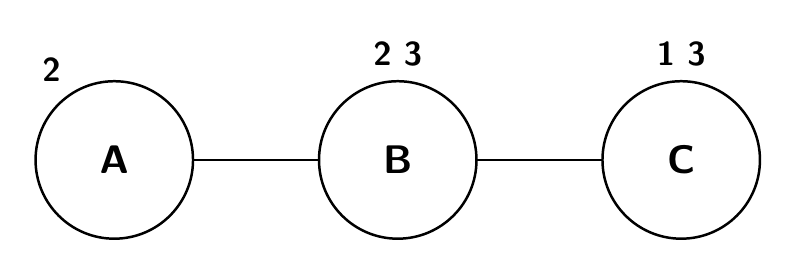
\begin{tikzpicture}[x=1mm, y=1mm]
\useasboundingbox (-11.0,-11.0) rectangle (83.0,16.8);
\draw[line width=0.9pt] (0.00,0.00) -- (36.00,0.00);
\draw[line width=0.9pt] (36.00,0.00) -- (72.00,0.00);
\draw[line width=0.9pt, fill=white] (0.00,0.00) circle (10.0mm);
\node[font=\Large\bfseries] at (0.00,0.00) {A};
\draw[line width=0.9pt, fill=white] (36.00,0.00) circle (10.0mm);
\node[font=\Large\bfseries] at (36.00,0.00) {B};
\draw[line width=0.9pt, fill=white] (72.00,0.00) circle (10.0mm);
\node[font=\Large\bfseries] at (72.00,0.00) {C};
\node[font=\large\bfseries, inner sep=0.5mm, anchor=305] at (-6.54,9.34) {2};
\node[font=\large\bfseries, inner sep=0.5mm, anchor=270] at (36.00,11.40) {2\,\,3};
\node[font=\large\bfseries, inner sep=0.5mm, anchor=270] at (72.00,11.40) {1\,\,3};
\end{tikzpicture} \hfill 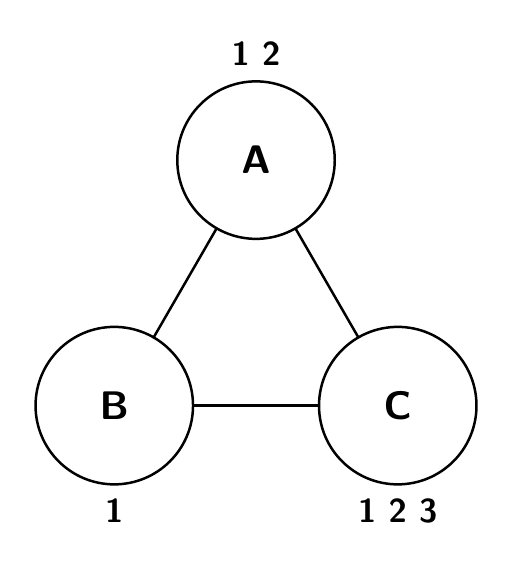
\begin{tikzpicture}[x=1mm, y=1mm]
\useasboundingbox (-29.0,-16.8) rectangle (29.0,48.0);
\draw[line width=0.9pt] (0.00,31.18) -- (-18.00,0.00);
\draw[line width=0.9pt] (-18.00,0.00) -- (18.00,0.00);
\draw[line width=0.9pt] (18.00,0.00) -- (0.00,31.18);
\draw[line width=0.9pt, fill=white] (0.00,31.18) circle (10.0mm);
\node[font=\Large\bfseries] at (0.00,31.18) {A};
\draw[line width=0.9pt, fill=white] (-18.00,0.00) circle (10.0mm);
\node[font=\Large\bfseries] at (-18.00,0.00) {B};
\draw[line width=0.9pt, fill=white] (18.00,0.00) circle (10.0mm);
\node[font=\Large\bfseries] at (18.00,0.00) {C};
\node[font=\large\bfseries, inner sep=0.5mm, anchor=270] at (0.00,42.58) {1\,\,2};
\node[font=\large\bfseries, inner sep=0.5mm, anchor=90] at (-18.00,-11.40) {1};
\node[font=\large\bfseries, inner sep=0.5mm, anchor=90] at (18.00,-11.40) {1\,\,2\,\,3};
\end{tikzpicture} \hfill}\par
\vspace{10mm}
\noindent\makebox[\linewidth][s]{\hfill 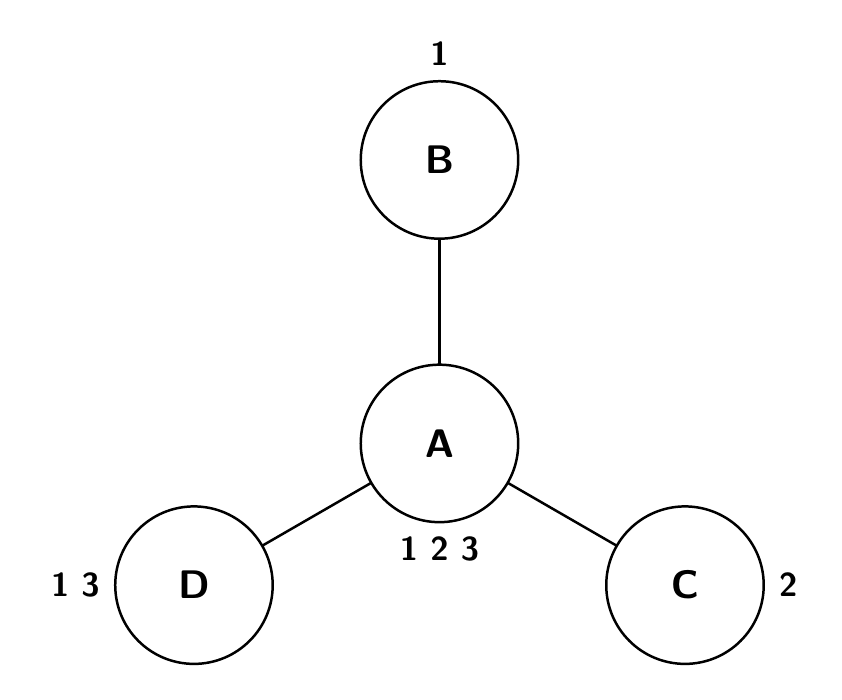
\begin{tikzpicture}[x=1mm, y=1mm]
\useasboundingbox (-52.3,-29.0) rectangle (47.5,52.8);
\draw[line width=0.9pt] (0.00,0.00) -- (0.00,36.00);
\draw[line width=0.9pt] (0.00,0.00) -- (31.18,-18.00);
\draw[line width=0.9pt] (0.00,0.00) -- (-31.18,-18.00);
\draw[line width=0.9pt, fill=white] (0.00,0.00) circle (10.0mm);
\node[font=\Large\bfseries] at (0.00,0.00) {A};
\draw[line width=0.9pt, fill=white] (0.00,36.00) circle (10.0mm);
\node[font=\Large\bfseries] at (0.00,36.00) {B};
\draw[line width=0.9pt, fill=white] (31.18,-18.00) circle (10.0mm);
\node[font=\Large\bfseries] at (31.18,-18.00) {C};
\draw[line width=0.9pt, fill=white] (-31.18,-18.00) circle (10.0mm);
\node[font=\Large\bfseries] at (-31.18,-18.00) {D};
\node[font=\large\bfseries, inner sep=0.5mm, anchor=90] at (-0.00,-11.40) {1\,\,2\,\,3};
\node[font=\large\bfseries, inner sep=0.5mm, anchor=270] at (0.00,47.40) {1};
\node[font=\large\bfseries, inner sep=0.5mm, anchor=180] at (42.58,-18.00) {2};
\node[font=\large\bfseries, inner sep=0.5mm, anchor=0] at (-42.58,-18.00) {1\,\,3};
\end{tikzpicture} \hfill 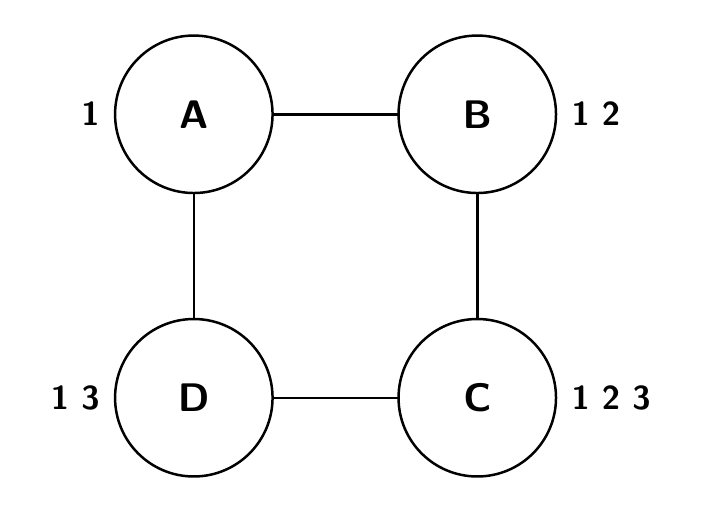
\begin{tikzpicture}[x=1mm, y=1mm]
\useasboundingbox (-21.1,-11.0) rectangle (61.9,47.0);
\draw[line width=0.9pt] (0.00,36.00) -- (36.00,36.00);
\draw[line width=0.9pt] (36.00,36.00) -- (36.00,0.00);
\draw[line width=0.9pt] (36.00,0.00) -- (0.00,0.00);
\draw[line width=0.9pt] (0.00,0.00) -- (0.00,36.00);
\draw[line width=0.9pt, fill=white] (0.00,36.00) circle (10.0mm);
\node[font=\Large\bfseries] at (0.00,36.00) {A};
\draw[line width=0.9pt, fill=white] (36.00,36.00) circle (10.0mm);
\node[font=\Large\bfseries] at (36.00,36.00) {B};
\draw[line width=0.9pt, fill=white] (36.00,0.00) circle (10.0mm);
\node[font=\Large\bfseries] at (36.00,0.00) {C};
\draw[line width=0.9pt, fill=white] (0.00,0.00) circle (10.0mm);
\node[font=\Large\bfseries] at (0.00,0.00) {D};
\node[font=\large\bfseries, inner sep=0.5mm, anchor=0] at (-11.40,36.00) {1};
\node[font=\large\bfseries, inner sep=0.5mm, anchor=180] at (47.40,36.00) {1\,\,2};
\node[font=\large\bfseries, inner sep=0.5mm, anchor=180] at (47.40,0.00) {1\,\,2\,\,3};
\node[font=\large\bfseries, inner sep=0.5mm, anchor=0] at (-11.40,0.00) {1\,\,3};
\end{tikzpicture} \hfill}\par
\newpage
\textbf{Problem 2:} Some of these can't be done. Find them and show why.\par
\vspace{10mm}
\noindent\makebox[\linewidth][s]{\hfill 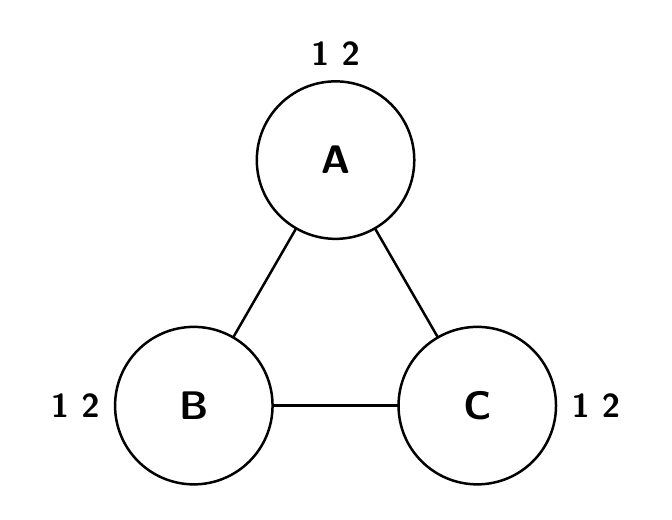
\begin{tikzpicture}[x=1mm, y=1mm]
\useasboundingbox (-39.1,-11.0) rectangle (39.1,48.0);
\draw[line width=0.9pt] (0.00,31.18) -- (-18.00,0.00);
\draw[line width=0.9pt] (-18.00,0.00) -- (18.00,0.00);
\draw[line width=0.9pt] (18.00,0.00) -- (0.00,31.18);
\draw[line width=0.9pt, fill=white] (0.00,31.18) circle (10.0mm);
\node[font=\Large\bfseries] at (0.00,31.18) {A};
\draw[line width=0.9pt, fill=white] (-18.00,0.00) circle (10.0mm);
\node[font=\Large\bfseries] at (-18.00,0.00) {B};
\draw[line width=0.9pt, fill=white] (18.00,0.00) circle (10.0mm);
\node[font=\Large\bfseries] at (18.00,0.00) {C};
\node[font=\large\bfseries, inner sep=0.5mm, anchor=270] at (0.00,42.58) {1\,\,2};
\node[font=\large\bfseries, inner sep=0.5mm, anchor=0] at (-29.40,0.00) {1\,\,2};
\node[font=\large\bfseries, inner sep=0.5mm, anchor=180] at (29.40,0.00) {1\,\,2};
\end{tikzpicture} \hfill 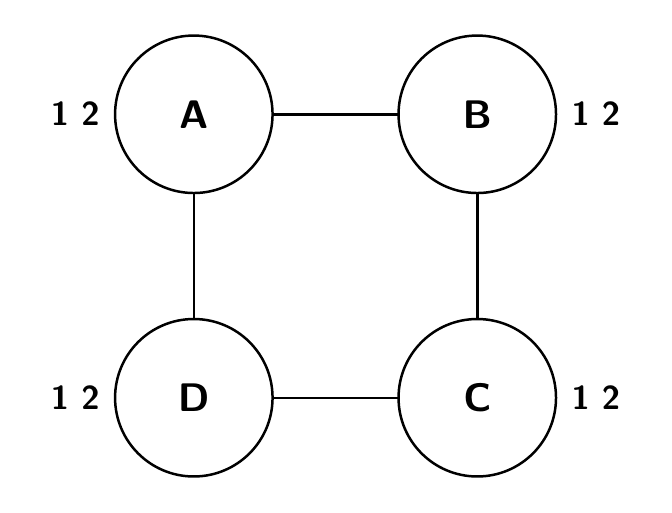
\begin{tikzpicture}[x=1mm, y=1mm]
\useasboundingbox (-21.1,-11.0) rectangle (57.1,47.0);
\draw[line width=0.9pt] (0.00,36.00) -- (36.00,36.00);
\draw[line width=0.9pt] (36.00,36.00) -- (36.00,0.00);
\draw[line width=0.9pt] (36.00,0.00) -- (0.00,0.00);
\draw[line width=0.9pt] (0.00,0.00) -- (0.00,36.00);
\draw[line width=0.9pt, fill=white] (0.00,36.00) circle (10.0mm);
\node[font=\Large\bfseries] at (0.00,36.00) {A};
\draw[line width=0.9pt, fill=white] (36.00,36.00) circle (10.0mm);
\node[font=\Large\bfseries] at (36.00,36.00) {B};
\draw[line width=0.9pt, fill=white] (36.00,0.00) circle (10.0mm);
\node[font=\Large\bfseries] at (36.00,0.00) {C};
\draw[line width=0.9pt, fill=white] (0.00,0.00) circle (10.0mm);
\node[font=\Large\bfseries] at (0.00,0.00) {D};
\node[font=\large\bfseries, inner sep=0.5mm, anchor=0] at (-11.40,36.00) {1\,\,2};
\node[font=\large\bfseries, inner sep=0.5mm, anchor=180] at (47.40,36.00) {1\,\,2};
\node[font=\large\bfseries, inner sep=0.5mm, anchor=180] at (47.40,0.00) {1\,\,2};
\node[font=\large\bfseries, inner sep=0.5mm, anchor=0] at (-11.40,0.00) {1\,\,2};
\end{tikzpicture} \hfill}\par
\vspace{18mm}
\noindent\makebox[\linewidth][c]{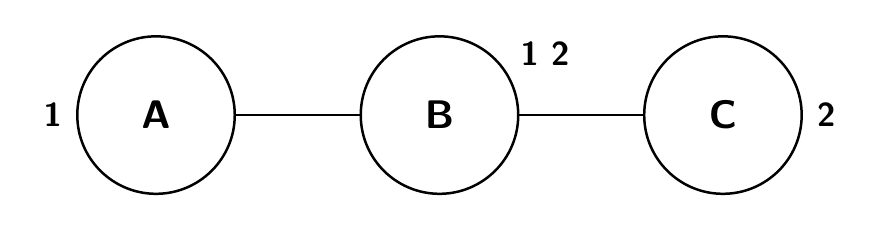
\begin{tikzpicture}[x=1mm, y=1mm]
\useasboundingbox (-16.3,-11.0) rectangle (88.3,11.1);
\draw[line width=0.9pt] (0.00,0.00) -- (36.00,0.00);
\draw[line width=0.9pt] (36.00,0.00) -- (72.00,0.00);
\draw[line width=0.9pt, fill=white] (0.00,0.00) circle (10.0mm);
\node[font=\Large\bfseries] at (0.00,0.00) {A};
\draw[line width=0.9pt, fill=white] (36.00,0.00) circle (10.0mm);
\node[font=\Large\bfseries] at (36.00,0.00) {B};
\draw[line width=0.9pt, fill=white] (72.00,0.00) circle (10.0mm);
\node[font=\Large\bfseries] at (72.00,0.00) {C};
\node[font=\large\bfseries, inner sep=0.5mm, anchor=0] at (-11.40,0.00) {1};
\node[font=\large\bfseries, inner sep=0.5mm, anchor=210] at (45.87,5.70) {1\,\,2};
\node[font=\large\bfseries, inner sep=0.5mm, anchor=180] at (83.40,0.00) {2};
\end{tikzpicture}}\par
\vspace{18mm}
\noindent\makebox[\linewidth][c]{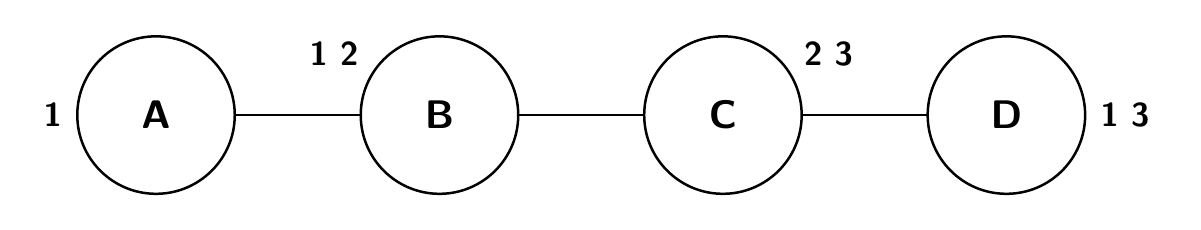
\begin{tikzpicture}[x=1mm, y=1mm]
\useasboundingbox (-16.3,-11.0) rectangle (129.1,11.1);
\draw[line width=0.9pt] (0.00,0.00) -- (36.00,0.00);
\draw[line width=0.9pt] (36.00,0.00) -- (72.00,0.00);
\draw[line width=0.9pt] (72.00,0.00) -- (108.00,0.00);
\draw[line width=0.9pt, fill=white] (0.00,0.00) circle (10.0mm);
\node[font=\Large\bfseries] at (0.00,0.00) {A};
\draw[line width=0.9pt, fill=white] (36.00,0.00) circle (10.0mm);
\node[font=\Large\bfseries] at (36.00,0.00) {B};
\draw[line width=0.9pt, fill=white] (72.00,0.00) circle (10.0mm);
\node[font=\Large\bfseries] at (72.00,0.00) {C};
\draw[line width=0.9pt, fill=white] (108.00,0.00) circle (10.0mm);
\node[font=\Large\bfseries] at (108.00,0.00) {D};
\node[font=\large\bfseries, inner sep=0.5mm, anchor=0] at (-11.40,0.00) {1};
\node[font=\large\bfseries, inner sep=0.5mm, anchor=330] at (26.13,5.70) {1\,\,2};
\node[font=\large\bfseries, inner sep=0.5mm, anchor=210] at (81.87,5.70) {2\,\,3};
\node[font=\large\bfseries, inner sep=0.5mm, anchor=180] at (119.40,0.00) {1\,\,3};
\end{tikzpicture}}\par
\newpage
\textbf{Problem 3:} Put a counter on every circle, or show why it can't be done.\par
\vspace{10mm}
\noindent\makebox[\linewidth][c]{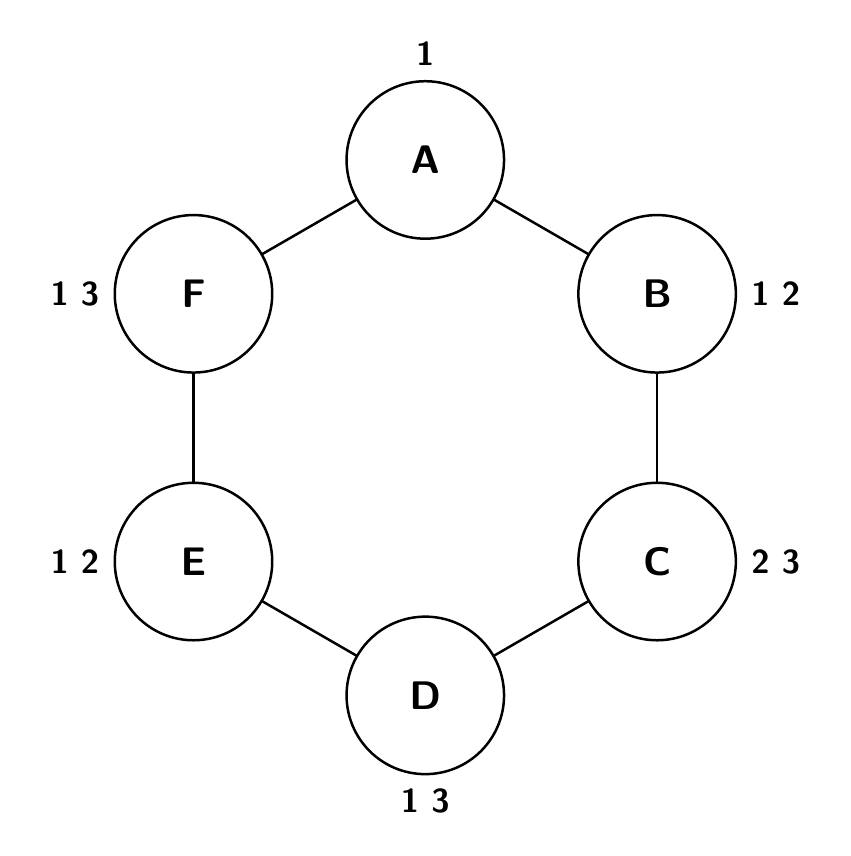
\begin{tikzpicture}[x=1mm, y=1mm]
\useasboundingbox (-50.5,-50.8) rectangle (50.5,50.8);
\draw[line width=0.9pt] (0.00,34.00) -- (29.44,17.00);
\draw[line width=0.9pt] (29.44,17.00) -- (29.44,-17.00);
\draw[line width=0.9pt] (29.44,-17.00) -- (0.00,-34.00);
\draw[line width=0.9pt] (0.00,-34.00) -- (-29.44,-17.00);
\draw[line width=0.9pt] (-29.44,-17.00) -- (-29.44,17.00);
\draw[line width=0.9pt] (-29.44,17.00) -- (0.00,34.00);
\draw[line width=0.9pt, fill=white] (0.00,34.00) circle (10.0mm);
\node[font=\Large\bfseries] at (0.00,34.00) {A};
\draw[line width=0.9pt, fill=white] (29.44,17.00) circle (10.0mm);
\node[font=\Large\bfseries] at (29.44,17.00) {B};
\draw[line width=0.9pt, fill=white] (29.44,-17.00) circle (10.0mm);
\node[font=\Large\bfseries] at (29.44,-17.00) {C};
\draw[line width=0.9pt, fill=white] (0.00,-34.00) circle (10.0mm);
\node[font=\Large\bfseries] at (0.00,-34.00) {D};
\draw[line width=0.9pt, fill=white] (-29.44,-17.00) circle (10.0mm);
\node[font=\Large\bfseries] at (-29.44,-17.00) {E};
\draw[line width=0.9pt, fill=white] (-29.44,17.00) circle (10.0mm);
\node[font=\Large\bfseries] at (-29.44,17.00) {F};
\node[font=\large\bfseries, inner sep=0.5mm, anchor=270] at (0.00,45.40) {1};
\node[font=\large\bfseries, inner sep=0.5mm, anchor=180] at (40.84,17.00) {1\,\,2};
\node[font=\large\bfseries, inner sep=0.5mm, anchor=180] at (40.84,-17.00) {2\,\,3};
\node[font=\large\bfseries, inner sep=0.5mm, anchor=90] at (-0.00,-45.40) {1\,\,3};
\node[font=\large\bfseries, inner sep=0.5mm, anchor=0] at (-40.84,-17.00) {1\,\,2};
\node[font=\large\bfseries, inner sep=0.5mm, anchor=0] at (-40.84,17.00) {1\,\,3};
\end{tikzpicture}}\par
\vspace{16mm}
\noindent\makebox[\linewidth][c]{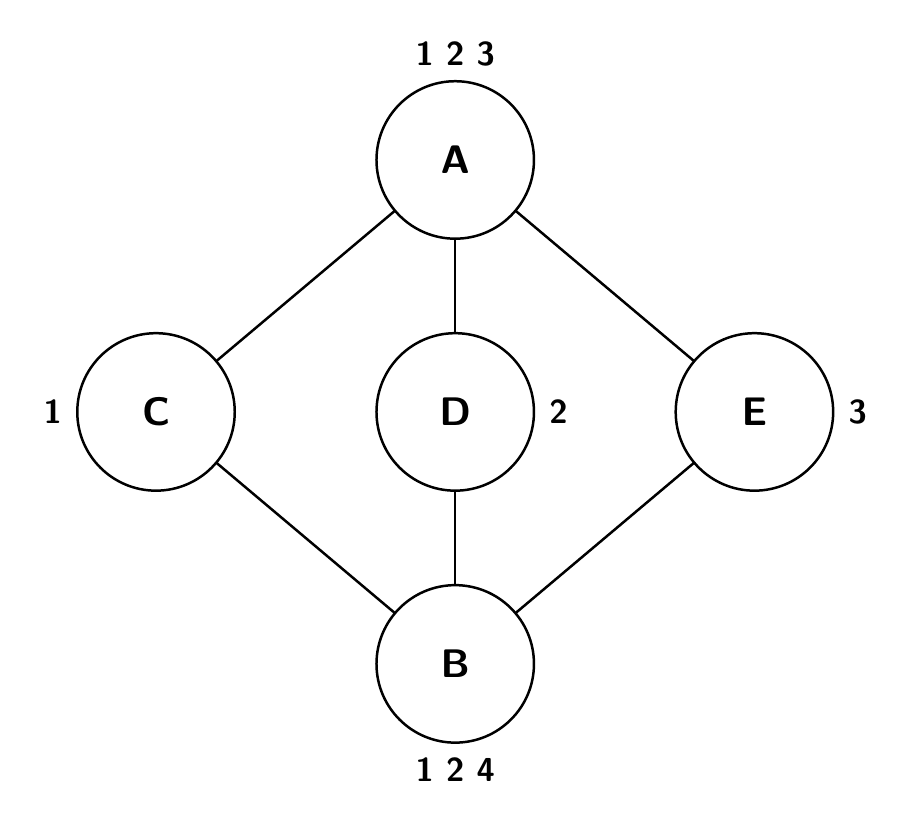
\begin{tikzpicture}[x=1mm, y=1mm]
\useasboundingbox (-54.3,-48.8) rectangle (54.3,48.8);
\draw[line width=0.9pt] (0.00,32.00) -- (-38.00,0.00);
\draw[line width=0.9pt] (0.00,32.00) -- (0.00,0.00);
\draw[line width=0.9pt] (0.00,32.00) -- (38.00,0.00);
\draw[line width=0.9pt] (0.00,-32.00) -- (-38.00,0.00);
\draw[line width=0.9pt] (0.00,-32.00) -- (0.00,0.00);
\draw[line width=0.9pt] (0.00,-32.00) -- (38.00,0.00);
\draw[line width=0.9pt, fill=white] (0.00,32.00) circle (10.0mm);
\node[font=\Large\bfseries] at (0.00,32.00) {A};
\draw[line width=0.9pt, fill=white] (0.00,-32.00) circle (10.0mm);
\node[font=\Large\bfseries] at (0.00,-32.00) {B};
\draw[line width=0.9pt, fill=white] (-38.00,0.00) circle (10.0mm);
\node[font=\Large\bfseries] at (-38.00,0.00) {C};
\draw[line width=0.9pt, fill=white] (0.00,0.00) circle (10.0mm);
\node[font=\Large\bfseries] at (0.00,0.00) {D};
\draw[line width=0.9pt, fill=white] (38.00,0.00) circle (10.0mm);
\node[font=\Large\bfseries] at (38.00,0.00) {E};
\node[font=\large\bfseries, inner sep=0.5mm, anchor=270] at (0.00,43.40) {1\,\,2\,\,3};
\node[font=\large\bfseries, inner sep=0.5mm, anchor=90] at (-0.00,-43.40) {1\,\,2\,\,4};
\node[font=\large\bfseries, inner sep=0.5mm, anchor=0] at (-49.40,0.00) {1};
\node[font=\large\bfseries, inner sep=0.5mm, anchor=180] at (11.40,0.00) {2};
\node[font=\large\bfseries, inner sep=0.5mm, anchor=180] at (49.40,0.00) {3};
\end{tikzpicture}}\par
\newpage
A move takes one counter off a circle and puts a counter with a different number there. After every move, circles joined by a line must still have different numbers.\par
\vspace{3mm}
\noindent\makebox[\linewidth][c]{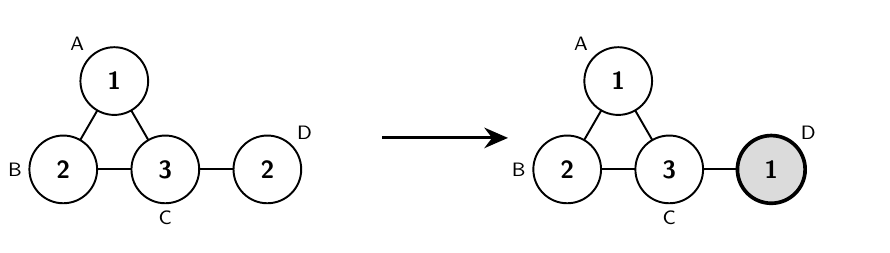
\begin{tikzpicture}[x=1mm, y=1mm]
\useasboundingbox (-11.0,-7.0) rectangle (95.0,18.0);
\draw[line width=0.7pt] (0.00,11.22) -- (-6.48,0.00);
\draw[line width=0.7pt] (-6.48,0.00) -- (6.48,0.00);
\draw[line width=0.7pt] (6.48,0.00) -- (0.00,11.22);
\draw[line width=0.7pt] (6.48,0.00) -- (19.44,0.00);
\draw[line width=0.7pt, fill=white] (0.00,11.22) circle (4.3mm);
\node[font=\small\bfseries] at (0.00,11.22) {1};
\node[font=\scriptsize, inner sep=0.4mm, anchor=315] at (-3.39,14.62) {A};
\draw[line width=0.7pt, fill=white] (-6.48,0.00) circle (4.3mm);
\node[font=\small\bfseries] at (-6.48,0.00) {2};
\node[font=\scriptsize, inner sep=0.4mm, anchor=0] at (-11.28,0.00) {B};
\draw[line width=0.7pt, fill=white] (6.48,0.00) circle (4.3mm);
\node[font=\small\bfseries] at (6.48,0.00) {3};
\node[font=\scriptsize, inner sep=0.4mm, anchor=90] at (6.48,-4.80) {C};
\draw[line width=0.7pt, fill=white] (19.44,0.00) circle (4.3mm);
\node[font=\small\bfseries] at (19.44,0.00) {2};
\node[font=\scriptsize, inner sep=0.4mm, anchor=225] at (22.83,3.39) {D};
\draw[bigarrow] (34.0,4) -- (50.0,4);
\draw[line width=0.7pt] (64.00,11.22) -- (57.52,0.00);
\draw[line width=0.7pt] (57.52,0.00) -- (70.48,0.00);
\draw[line width=0.7pt] (70.48,0.00) -- (64.00,11.22);
\draw[line width=0.7pt] (70.48,0.00) -- (83.44,0.00);
\draw[line width=0.7pt, fill=white] (64.00,11.22) circle (4.3mm);
\node[font=\small\bfseries] at (64.00,11.22) {1};
\node[font=\scriptsize, inner sep=0.4mm, anchor=315] at (60.61,14.62) {A};
\draw[line width=0.7pt, fill=white] (57.52,0.00) circle (4.3mm);
\node[font=\small\bfseries] at (57.52,0.00) {2};
\node[font=\scriptsize, inner sep=0.4mm, anchor=0] at (52.72,0.00) {B};
\draw[line width=0.7pt, fill=white] (70.48,0.00) circle (4.3mm);
\node[font=\small\bfseries] at (70.48,0.00) {3};
\node[font=\scriptsize, inner sep=0.4mm, anchor=90] at (70.48,-4.80) {C};
\draw[line width=1.3299999999999998pt, fill=black!14] (83.44,0.00) circle (4.3mm);
\node[font=\small\bfseries] at (83.44,0.00) {1};
\node[font=\scriptsize, inner sep=0.4mm, anchor=225] at (86.83,3.39) {D};
\end{tikzpicture}}\par
\vspace{4mm}
\textbf{Problem 4:} Set up Start. Can you change it into Goal one move at a time, using only the counters shown?\par
\vspace{5mm}
\noindent\makebox[\linewidth][c]{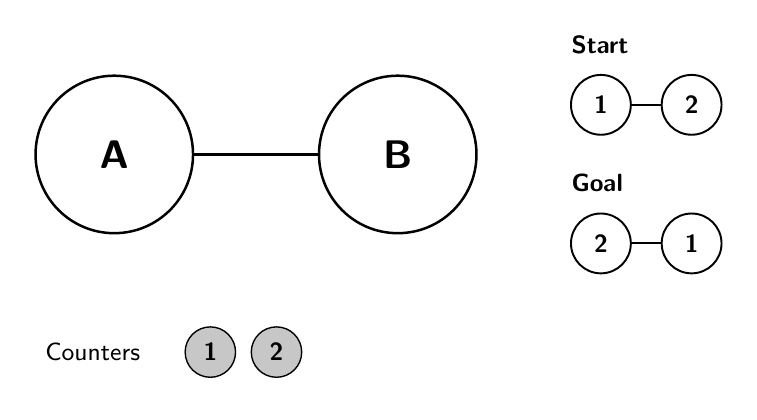
\begin{tikzpicture}[x=1mm, y=1mm]
\useasboundingbox (-11.0,-30.1) rectangle (78.1,16.1);
\draw[line width=0.9pt] (0.00,0.00) -- (36.00,0.00);
\draw[line width=0.9pt, fill=white] (0.00,0.00) circle (10.0mm);
\node[font=\Large\bfseries] at (0.00,0.00) {A};
\draw[line width=0.9pt, fill=white] (36.00,0.00) circle (10.0mm);
\node[font=\Large\bfseries] at (36.00,0.00) {B};
\node[anchor=north west, font=\small\bfseries, inner sep=0] at (58.0,15.1) {Start};
\draw[line width=0.7pt] (61.80,6.30) -- (73.32,6.30);
\draw[line width=0.7pt, fill=white] (61.80,6.30) circle (3.8mm);
\node[font=\small\bfseries] at (61.80,6.30) {1};
\draw[line width=0.7pt, fill=white] (73.32,6.30) circle (3.8mm);
\node[font=\small\bfseries] at (73.32,6.30) {2};
\node[anchor=north west, font=\small\bfseries, inner sep=0] at (58.0,-2.5) {Goal};
\draw[line width=0.7pt] (61.80,-11.30) -- (73.32,-11.30);
\draw[line width=0.7pt, fill=white] (61.80,-11.30) circle (3.8mm);
\node[font=\small\bfseries] at (61.80,-11.30) {2};
\draw[line width=0.7pt, fill=white] (73.32,-11.30) circle (3.8mm);
\node[font=\small\bfseries] at (73.32,-11.30) {1};
\node[anchor=west, font=\small] at (-10.0,-25.1) {Counters};
\draw[line width=0.5pt, fill=black!22] (12.2,-25.1) circle (3.2mm);
\node[font=\small\bfseries] at (12.2,-25.1) {1};
\draw[line width=0.5pt, fill=black!22] (20.6,-25.1) circle (3.2mm);
\node[font=\small\bfseries] at (20.6,-25.1) {2};
\end{tikzpicture}}\par
\vspace{9mm}
\noindent\makebox[\linewidth][c]{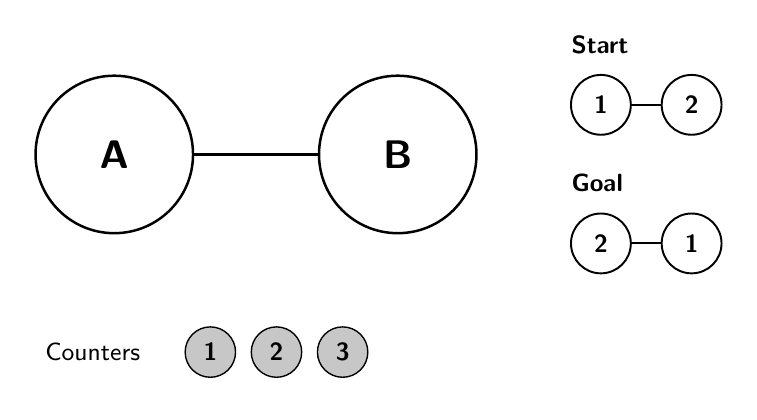
\begin{tikzpicture}[x=1mm, y=1mm]
\useasboundingbox (-11.0,-30.1) rectangle (78.1,16.1);
\draw[line width=0.9pt] (0.00,0.00) -- (36.00,0.00);
\draw[line width=0.9pt, fill=white] (0.00,0.00) circle (10.0mm);
\node[font=\Large\bfseries] at (0.00,0.00) {A};
\draw[line width=0.9pt, fill=white] (36.00,0.00) circle (10.0mm);
\node[font=\Large\bfseries] at (36.00,0.00) {B};
\node[anchor=north west, font=\small\bfseries, inner sep=0] at (58.0,15.1) {Start};
\draw[line width=0.7pt] (61.80,6.30) -- (73.32,6.30);
\draw[line width=0.7pt, fill=white] (61.80,6.30) circle (3.8mm);
\node[font=\small\bfseries] at (61.80,6.30) {1};
\draw[line width=0.7pt, fill=white] (73.32,6.30) circle (3.8mm);
\node[font=\small\bfseries] at (73.32,6.30) {2};
\node[anchor=north west, font=\small\bfseries, inner sep=0] at (58.0,-2.5) {Goal};
\draw[line width=0.7pt] (61.80,-11.30) -- (73.32,-11.30);
\draw[line width=0.7pt, fill=white] (61.80,-11.30) circle (3.8mm);
\node[font=\small\bfseries] at (61.80,-11.30) {2};
\draw[line width=0.7pt, fill=white] (73.32,-11.30) circle (3.8mm);
\node[font=\small\bfseries] at (73.32,-11.30) {1};
\node[anchor=west, font=\small] at (-10.0,-25.1) {Counters};
\draw[line width=0.5pt, fill=black!22] (12.2,-25.1) circle (3.2mm);
\node[font=\small\bfseries] at (12.2,-25.1) {1};
\draw[line width=0.5pt, fill=black!22] (20.6,-25.1) circle (3.2mm);
\node[font=\small\bfseries] at (20.6,-25.1) {2};
\draw[line width=0.5pt, fill=black!22] (29.0,-25.1) circle (3.2mm);
\node[font=\small\bfseries] at (29.0,-25.1) {3};
\end{tikzpicture}}\par
\vspace{12mm}
\textbf{Problem 5:} Set up Start, then change it into Goal in as few moves as you can.\par
\vspace{5mm}
\noindent\makebox[\linewidth][c]{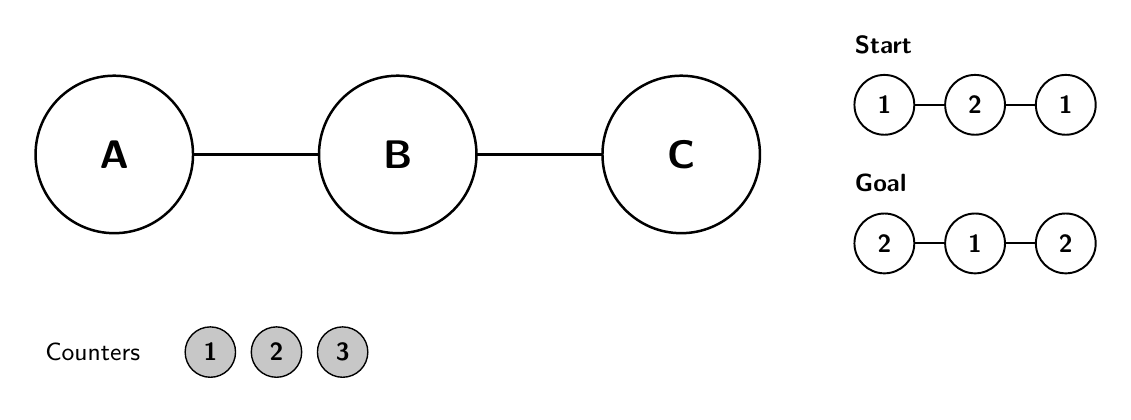
\begin{tikzpicture}[x=1mm, y=1mm]
\useasboundingbox (-11.0,-30.1) rectangle (125.6,16.1);
\draw[line width=0.9pt] (0.00,0.00) -- (36.00,0.00);
\draw[line width=0.9pt] (36.00,0.00) -- (72.00,0.00);
\draw[line width=0.9pt, fill=white] (0.00,0.00) circle (10.0mm);
\node[font=\Large\bfseries] at (0.00,0.00) {A};
\draw[line width=0.9pt, fill=white] (36.00,0.00) circle (10.0mm);
\node[font=\Large\bfseries] at (36.00,0.00) {B};
\draw[line width=0.9pt, fill=white] (72.00,0.00) circle (10.0mm);
\node[font=\Large\bfseries] at (72.00,0.00) {C};
\node[anchor=north west, font=\small\bfseries, inner sep=0] at (94.0,15.1) {Start};
\draw[line width=0.7pt] (97.80,6.30) -- (109.32,6.30);
\draw[line width=0.7pt] (109.32,6.30) -- (120.84,6.30);
\draw[line width=0.7pt, fill=white] (97.80,6.30) circle (3.8mm);
\node[font=\small\bfseries] at (97.80,6.30) {1};
\draw[line width=0.7pt, fill=white] (109.32,6.30) circle (3.8mm);
\node[font=\small\bfseries] at (109.32,6.30) {2};
\draw[line width=0.7pt, fill=white] (120.84,6.30) circle (3.8mm);
\node[font=\small\bfseries] at (120.84,6.30) {1};
\node[anchor=north west, font=\small\bfseries, inner sep=0] at (94.0,-2.5) {Goal};
\draw[line width=0.7pt] (97.80,-11.30) -- (109.32,-11.30);
\draw[line width=0.7pt] (109.32,-11.30) -- (120.84,-11.30);
\draw[line width=0.7pt, fill=white] (97.80,-11.30) circle (3.8mm);
\node[font=\small\bfseries] at (97.80,-11.30) {2};
\draw[line width=0.7pt, fill=white] (109.32,-11.30) circle (3.8mm);
\node[font=\small\bfseries] at (109.32,-11.30) {1};
\draw[line width=0.7pt, fill=white] (120.84,-11.30) circle (3.8mm);
\node[font=\small\bfseries] at (120.84,-11.30) {2};
\node[anchor=west, font=\small] at (-10.0,-25.1) {Counters};
\draw[line width=0.5pt, fill=black!22] (12.2,-25.1) circle (3.2mm);
\node[font=\small\bfseries] at (12.2,-25.1) {1};
\draw[line width=0.5pt, fill=black!22] (20.6,-25.1) circle (3.2mm);
\node[font=\small\bfseries] at (20.6,-25.1) {2};
\draw[line width=0.5pt, fill=black!22] (29.0,-25.1) circle (3.2mm);
\node[font=\small\bfseries] at (29.0,-25.1) {3};
\end{tikzpicture}}\par
\newpage
\textbf{Problem 6:} Set up Start, then change it into Goal in as few moves as you can.\par
\vspace{5mm}
\noindent\makebox[\linewidth][c]{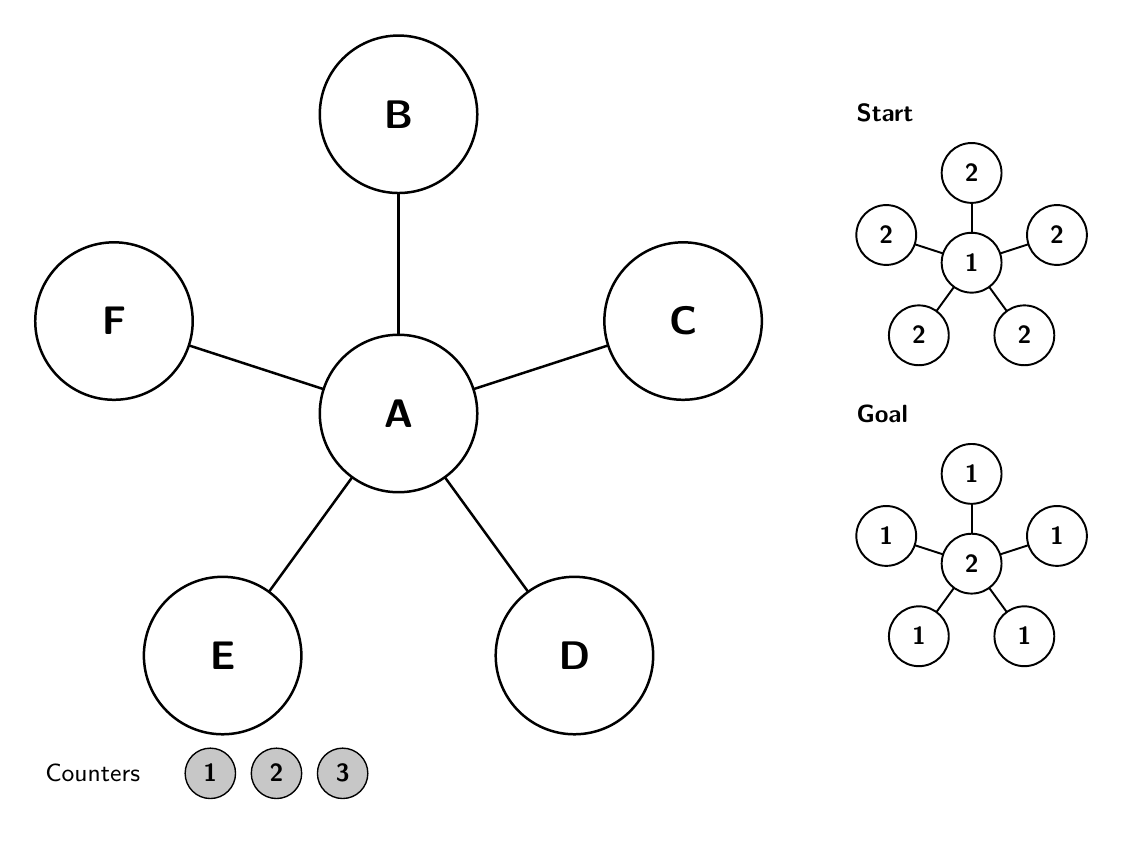
\begin{tikzpicture}[x=1mm, y=1mm]
\useasboundingbox (-47.1,-50.7) rectangle (88.4,49.0);
\draw[line width=0.9pt] (0.00,0.00) -- (0.00,38.00);
\draw[line width=0.9pt] (0.00,0.00) -- (36.14,11.74);
\draw[line width=0.9pt] (0.00,0.00) -- (22.34,-30.74);
\draw[line width=0.9pt] (0.00,0.00) -- (-22.34,-30.74);
\draw[line width=0.9pt] (0.00,0.00) -- (-36.14,11.74);
\draw[line width=0.9pt, fill=white] (0.00,0.00) circle (10.0mm);
\node[font=\Large\bfseries] at (0.00,0.00) {A};
\draw[line width=0.9pt, fill=white] (0.00,38.00) circle (10.0mm);
\node[font=\Large\bfseries] at (0.00,38.00) {B};
\draw[line width=0.9pt, fill=white] (36.14,11.74) circle (10.0mm);
\node[font=\Large\bfseries] at (36.14,11.74) {C};
\draw[line width=0.9pt, fill=white] (22.34,-30.74) circle (10.0mm);
\node[font=\Large\bfseries] at (22.34,-30.74) {D};
\draw[line width=0.9pt, fill=white] (-22.34,-30.74) circle (10.0mm);
\node[font=\Large\bfseries] at (-22.34,-30.74) {E};
\draw[line width=0.9pt, fill=white] (-36.14,11.74) circle (10.0mm);
\node[font=\Large\bfseries] at (-36.14,11.74) {F};
\node[anchor=north west, font=\small\bfseries, inner sep=0] at (58.1,39.4) {Start};
\draw[line width=0.7pt] (72.78,19.15) -- (72.78,30.55);
\draw[line width=0.7pt] (72.78,19.15) -- (83.62,22.67);
\draw[line width=0.7pt] (72.78,19.15) -- (79.48,9.93);
\draw[line width=0.7pt] (72.78,19.15) -- (66.08,9.93);
\draw[line width=0.7pt] (72.78,19.15) -- (61.94,22.67);
\draw[line width=0.7pt, fill=white] (72.78,19.15) circle (3.8mm);
\node[font=\small\bfseries] at (72.78,19.15) {1};
\draw[line width=0.7pt, fill=white] (72.78,30.55) circle (3.8mm);
\node[font=\small\bfseries] at (72.78,30.55) {2};
\draw[line width=0.7pt, fill=white] (83.62,22.67) circle (3.8mm);
\node[font=\small\bfseries] at (83.62,22.67) {2};
\draw[line width=0.7pt, fill=white] (79.48,9.93) circle (3.8mm);
\node[font=\small\bfseries] at (79.48,9.93) {2};
\draw[line width=0.7pt, fill=white] (66.08,9.93) circle (3.8mm);
\node[font=\small\bfseries] at (66.08,9.93) {2};
\draw[line width=0.7pt, fill=white] (61.94,22.67) circle (3.8mm);
\node[font=\small\bfseries] at (61.94,22.67) {2};
\node[anchor=north west, font=\small\bfseries, inner sep=0] at (58.1,1.1) {Goal};
\draw[line width=0.7pt] (72.78,-19.07) -- (72.78,-7.67);
\draw[line width=0.7pt] (72.78,-19.07) -- (83.62,-15.55);
\draw[line width=0.7pt] (72.78,-19.07) -- (79.48,-28.29);
\draw[line width=0.7pt] (72.78,-19.07) -- (66.08,-28.29);
\draw[line width=0.7pt] (72.78,-19.07) -- (61.94,-15.55);
\draw[line width=0.7pt, fill=white] (72.78,-19.07) circle (3.8mm);
\node[font=\small\bfseries] at (72.78,-19.07) {2};
\draw[line width=0.7pt, fill=white] (72.78,-7.67) circle (3.8mm);
\node[font=\small\bfseries] at (72.78,-7.67) {1};
\draw[line width=0.7pt, fill=white] (83.62,-15.55) circle (3.8mm);
\node[font=\small\bfseries] at (83.62,-15.55) {1};
\draw[line width=0.7pt, fill=white] (79.48,-28.29) circle (3.8mm);
\node[font=\small\bfseries] at (79.48,-28.29) {1};
\draw[line width=0.7pt, fill=white] (66.08,-28.29) circle (3.8mm);
\node[font=\small\bfseries] at (66.08,-28.29) {1};
\draw[line width=0.7pt, fill=white] (61.94,-15.55) circle (3.8mm);
\node[font=\small\bfseries] at (61.94,-15.55) {1};
\node[anchor=west, font=\small] at (-46.1,-45.7) {Counters};
\draw[line width=0.5pt, fill=black!22] (-23.9,-45.7) circle (3.2mm);
\node[font=\small\bfseries] at (-23.9,-45.7) {1};
\draw[line width=0.5pt, fill=black!22] (-15.5,-45.7) circle (3.2mm);
\node[font=\small\bfseries] at (-15.5,-45.7) {2};
\draw[line width=0.5pt, fill=black!22] (-7.1,-45.7) circle (3.2mm);
\node[font=\small\bfseries] at (-7.1,-45.7) {3};
\end{tikzpicture}}\par
\vspace{14mm}
\textbf{Problem 7:} Set up Start, then change it into Goal in as few moves as you can.\par
\vspace{5mm}
\noindent\makebox[\linewidth][c]{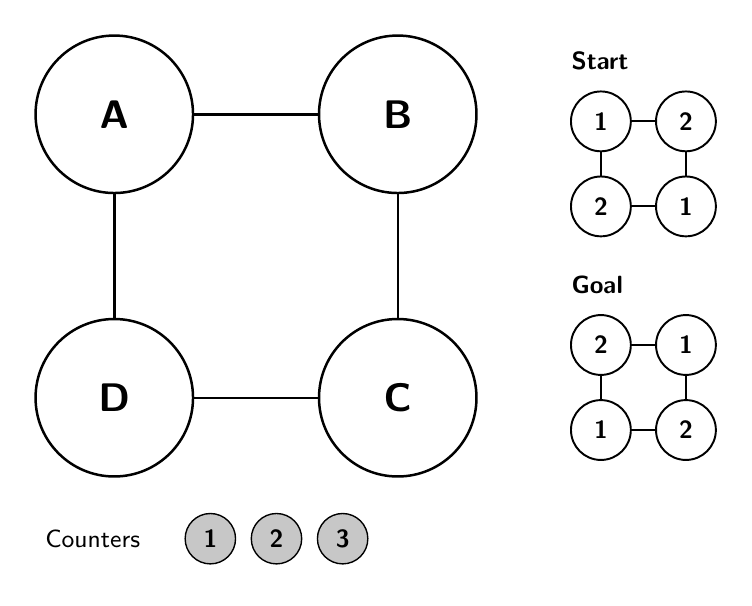
\begin{tikzpicture}[x=1mm, y=1mm]
\useasboundingbox (-11.0,-22.9) rectangle (77.4,47.0);
\draw[line width=0.9pt] (0.00,36.00) -- (36.00,36.00);
\draw[line width=0.9pt] (36.00,36.00) -- (36.00,0.00);
\draw[line width=0.9pt] (36.00,0.00) -- (0.00,0.00);
\draw[line width=0.9pt] (0.00,0.00) -- (0.00,36.00);
\draw[line width=0.9pt, fill=white] (0.00,36.00) circle (10.0mm);
\node[font=\Large\bfseries] at (0.00,36.00) {A};
\draw[line width=0.9pt, fill=white] (36.00,36.00) circle (10.0mm);
\node[font=\Large\bfseries] at (36.00,36.00) {B};
\draw[line width=0.9pt, fill=white] (36.00,0.00) circle (10.0mm);
\node[font=\Large\bfseries] at (36.00,0.00) {C};
\draw[line width=0.9pt, fill=white] (0.00,0.00) circle (10.0mm);
\node[font=\Large\bfseries] at (0.00,0.00) {D};
\node[anchor=north west, font=\small\bfseries, inner sep=0] at (58.0,43.9) {Start};
\draw[line width=0.7pt] (61.80,35.10) -- (72.60,35.10);
\draw[line width=0.7pt] (72.60,35.10) -- (72.60,24.30);
\draw[line width=0.7pt] (72.60,24.30) -- (61.80,24.30);
\draw[line width=0.7pt] (61.80,24.30) -- (61.80,35.10);
\draw[line width=0.7pt, fill=white] (61.80,35.10) circle (3.8mm);
\node[font=\small\bfseries] at (61.80,35.10) {1};
\draw[line width=0.7pt, fill=white] (72.60,35.10) circle (3.8mm);
\node[font=\small\bfseries] at (72.60,35.10) {2};
\draw[line width=0.7pt, fill=white] (72.60,24.30) circle (3.8mm);
\node[font=\small\bfseries] at (72.60,24.30) {1};
\draw[line width=0.7pt, fill=white] (61.80,24.30) circle (3.8mm);
\node[font=\small\bfseries] at (61.80,24.30) {2};
\node[anchor=north west, font=\small\bfseries, inner sep=0] at (58.0,15.5) {Goal};
\draw[line width=0.7pt] (61.80,6.70) -- (72.60,6.70);
\draw[line width=0.7pt] (72.60,6.70) -- (72.60,-4.10);
\draw[line width=0.7pt] (72.60,-4.10) -- (61.80,-4.10);
\draw[line width=0.7pt] (61.80,-4.10) -- (61.80,6.70);
\draw[line width=0.7pt, fill=white] (61.80,6.70) circle (3.8mm);
\node[font=\small\bfseries] at (61.80,6.70) {2};
\draw[line width=0.7pt, fill=white] (72.60,6.70) circle (3.8mm);
\node[font=\small\bfseries] at (72.60,6.70) {1};
\draw[line width=0.7pt, fill=white] (72.60,-4.10) circle (3.8mm);
\node[font=\small\bfseries] at (72.60,-4.10) {2};
\draw[line width=0.7pt, fill=white] (61.80,-4.10) circle (3.8mm);
\node[font=\small\bfseries] at (61.80,-4.10) {1};
\node[anchor=west, font=\small] at (-10.0,-17.9) {Counters};
\draw[line width=0.5pt, fill=black!22] (12.2,-17.9) circle (3.2mm);
\node[font=\small\bfseries] at (12.2,-17.9) {1};
\draw[line width=0.5pt, fill=black!22] (20.6,-17.9) circle (3.2mm);
\node[font=\small\bfseries] at (20.6,-17.9) {2};
\draw[line width=0.5pt, fill=black!22] (29.0,-17.9) circle (3.2mm);
\node[font=\small\bfseries] at (29.0,-17.9) {3};
\end{tikzpicture}}\par
\newpage
\textbf{Problem 8:} Set up Start. Can you change it into Goal one move at a time, using only the counters shown?\par
\vspace{12mm}
\noindent\makebox[\linewidth][c]{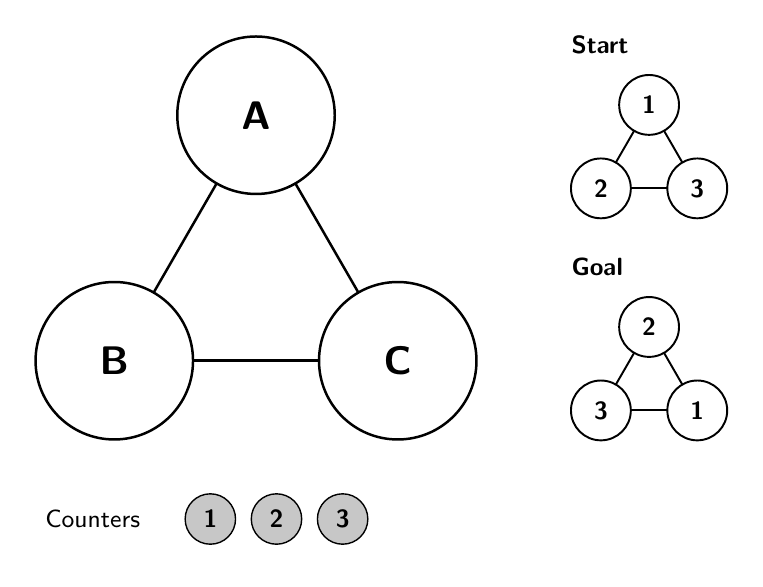
\begin{tikzpicture}[x=1mm, y=1mm]
\useasboundingbox (-29.0,-25.1) rectangle (60.8,42.3);
\draw[line width=0.9pt] (0.00,31.18) -- (-18.00,0.00);
\draw[line width=0.9pt] (-18.00,0.00) -- (18.00,0.00);
\draw[line width=0.9pt] (18.00,0.00) -- (0.00,31.18);
\draw[line width=0.9pt, fill=white] (0.00,31.18) circle (10.0mm);
\node[font=\Large\bfseries] at (0.00,31.18) {A};
\draw[line width=0.9pt, fill=white] (-18.00,0.00) circle (10.0mm);
\node[font=\Large\bfseries] at (-18.00,0.00) {B};
\draw[line width=0.9pt, fill=white] (18.00,0.00) circle (10.0mm);
\node[font=\Large\bfseries] at (18.00,0.00) {C};
\node[anchor=north west, font=\small\bfseries, inner sep=0] at (40.0,41.3) {Start};
\draw[line width=0.7pt] (49.92,32.49) -- (43.80,21.89);
\draw[line width=0.7pt] (43.80,21.89) -- (56.04,21.89);
\draw[line width=0.7pt] (56.04,21.89) -- (49.92,32.49);
\draw[line width=0.7pt, fill=white] (49.92,32.49) circle (3.8mm);
\node[font=\small\bfseries] at (49.92,32.49) {1};
\draw[line width=0.7pt, fill=white] (43.80,21.89) circle (3.8mm);
\node[font=\small\bfseries] at (43.80,21.89) {2};
\draw[line width=0.7pt, fill=white] (56.04,21.89) circle (3.8mm);
\node[font=\small\bfseries] at (56.04,21.89) {3};
\node[anchor=north west, font=\small\bfseries, inner sep=0] at (40.0,13.1) {Goal};
\draw[line width=0.7pt] (49.92,4.29) -- (43.80,-6.31);
\draw[line width=0.7pt] (43.80,-6.31) -- (56.04,-6.31);
\draw[line width=0.7pt] (56.04,-6.31) -- (49.92,4.29);
\draw[line width=0.7pt, fill=white] (49.92,4.29) circle (3.8mm);
\node[font=\small\bfseries] at (49.92,4.29) {2};
\draw[line width=0.7pt, fill=white] (43.80,-6.31) circle (3.8mm);
\node[font=\small\bfseries] at (43.80,-6.31) {3};
\draw[line width=0.7pt, fill=white] (56.04,-6.31) circle (3.8mm);
\node[font=\small\bfseries] at (56.04,-6.31) {1};
\node[anchor=west, font=\small] at (-28.0,-20.1) {Counters};
\draw[line width=0.5pt, fill=black!22] (-5.8,-20.1) circle (3.2mm);
\node[font=\small\bfseries] at (-5.8,-20.1) {1};
\draw[line width=0.5pt, fill=black!22] (2.6,-20.1) circle (3.2mm);
\node[font=\small\bfseries] at (2.6,-20.1) {2};
\draw[line width=0.5pt, fill=black!22] (11.0,-20.1) circle (3.2mm);
\node[font=\small\bfseries] at (11.0,-20.1) {3};
\end{tikzpicture}}\par
\vspace{20mm}
\noindent\makebox[\linewidth][c]{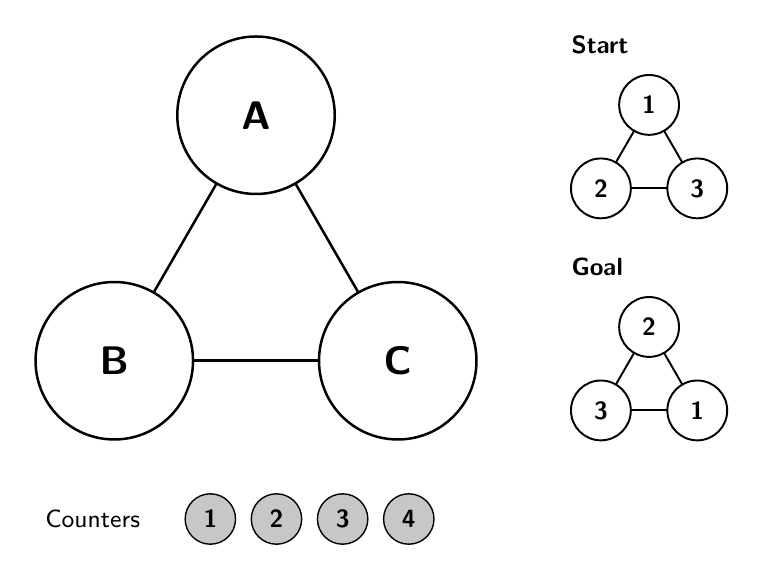
\begin{tikzpicture}[x=1mm, y=1mm]
\useasboundingbox (-29.0,-25.1) rectangle (60.8,42.3);
\draw[line width=0.9pt] (0.00,31.18) -- (-18.00,0.00);
\draw[line width=0.9pt] (-18.00,0.00) -- (18.00,0.00);
\draw[line width=0.9pt] (18.00,0.00) -- (0.00,31.18);
\draw[line width=0.9pt, fill=white] (0.00,31.18) circle (10.0mm);
\node[font=\Large\bfseries] at (0.00,31.18) {A};
\draw[line width=0.9pt, fill=white] (-18.00,0.00) circle (10.0mm);
\node[font=\Large\bfseries] at (-18.00,0.00) {B};
\draw[line width=0.9pt, fill=white] (18.00,0.00) circle (10.0mm);
\node[font=\Large\bfseries] at (18.00,0.00) {C};
\node[anchor=north west, font=\small\bfseries, inner sep=0] at (40.0,41.3) {Start};
\draw[line width=0.7pt] (49.92,32.49) -- (43.80,21.89);
\draw[line width=0.7pt] (43.80,21.89) -- (56.04,21.89);
\draw[line width=0.7pt] (56.04,21.89) -- (49.92,32.49);
\draw[line width=0.7pt, fill=white] (49.92,32.49) circle (3.8mm);
\node[font=\small\bfseries] at (49.92,32.49) {1};
\draw[line width=0.7pt, fill=white] (43.80,21.89) circle (3.8mm);
\node[font=\small\bfseries] at (43.80,21.89) {2};
\draw[line width=0.7pt, fill=white] (56.04,21.89) circle (3.8mm);
\node[font=\small\bfseries] at (56.04,21.89) {3};
\node[anchor=north west, font=\small\bfseries, inner sep=0] at (40.0,13.1) {Goal};
\draw[line width=0.7pt] (49.92,4.29) -- (43.80,-6.31);
\draw[line width=0.7pt] (43.80,-6.31) -- (56.04,-6.31);
\draw[line width=0.7pt] (56.04,-6.31) -- (49.92,4.29);
\draw[line width=0.7pt, fill=white] (49.92,4.29) circle (3.8mm);
\node[font=\small\bfseries] at (49.92,4.29) {2};
\draw[line width=0.7pt, fill=white] (43.80,-6.31) circle (3.8mm);
\node[font=\small\bfseries] at (43.80,-6.31) {3};
\draw[line width=0.7pt, fill=white] (56.04,-6.31) circle (3.8mm);
\node[font=\small\bfseries] at (56.04,-6.31) {1};
\node[anchor=west, font=\small] at (-28.0,-20.1) {Counters};
\draw[line width=0.5pt, fill=black!22] (-5.8,-20.1) circle (3.2mm);
\node[font=\small\bfseries] at (-5.8,-20.1) {1};
\draw[line width=0.5pt, fill=black!22] (2.6,-20.1) circle (3.2mm);
\node[font=\small\bfseries] at (2.6,-20.1) {2};
\draw[line width=0.5pt, fill=black!22] (11.0,-20.1) circle (3.2mm);
\node[font=\small\bfseries] at (11.0,-20.1) {3};
\draw[line width=0.5pt, fill=black!22] (19.4,-20.1) circle (3.2mm);
\node[font=\small\bfseries] at (19.4,-20.1) {4};
\end{tikzpicture}}\par
\end{document}
